\lysh{33892}{4}

\begin{alist}
\item Το τριώνυμο $x^2 + x - 6$ έχει διακρίνουσα $\Delta = 1^2 - 4 \cdot 1 \cdot (-6) = 25 > 0$. Το άθροισμα των
ριζών του είναι $S = \dfrac{-1}{1} = -1$ και το γινόμενό τους είναι $P = \dfrac{-6}{1} = -6$, οπότε οι ρίζες είναι
$x_1 = -3$ και $x_2 = 2$. Το πρόσημο του τριωνύμου φαίνεται στον παρακάτω πίνακα:

\begin{center}
\begin{tikzpicture}
\tikzset{t style/.style = {style = dashed}}
\tkzTabInit[color,lgt=3,espcl=2,colorC = maincolor!40,
colorL = maincolor!20,
colorV = maincolor!40]%
{$x$ / .8,$x^2 + x - 6$ /0.8}%
{$-\infty$,$-3$,$2$,$+\infty$}%
\tkzTabLine{ , $+$, z
, $-$ , z
, $+$ , }
\end{tikzpicture}
\end{center}

Οπότε η ανίσωση $x^2 + x - 6 < 0$ αληθεύει για $x \in (-3, 2)$.

\item Έχουμε ισοδύναμα:
\begin{gather*}
\left|x - \dfrac{1}{2}\right| > 1\text{, δηλαδή} \\
x - \dfrac{1}{2} < -1 \text{ ή } x - \dfrac{1}{2} > 1\text{και τελικά} \\
x < -\dfrac{1}{2} \text{ ή } x > \dfrac{3}{2}.
\end{gather*}

\item 
\begin{rlist}
\item Ο αριθμός $\alpha$ ικανοποιεί τη σχέση $\left|\alpha - \dfrac{1}{2}\right| > 1$, οπότε από το $\beta)$ ερώτημα $\alpha < -\dfrac{1}{2}$
(απορρίπτονται οι τιμές αυτές γιατί $\alpha > 0$, ως πλευρά) ή $\alpha > \dfrac{3}{2}$ (1).

Για το εμβαδόν $E$ του ορθογωνίου ισχύει $E < 6 \Leftrightarrow \alpha \cdot (\alpha + 1) < 6 \Leftrightarrow \alpha^2 + \alpha - 6 < 0$. Από
το $\alpha)$ ερώτημα και επειδή $\alpha > 0$, η ανίσωση αληθεύει για $\alpha \in (0, 2)$ (2).

Από τις σχέσεις (1) και (2) προκύπτει $\dfrac{3}{2} < \alpha < 2$.

\item Η περίμετρος του ορθογωνίου είναι $\Pi = 2\alpha + 2(\alpha + 1) = 4\alpha + 2$.

Έχουμε $\dfrac{3}{2} < \alpha < 2 \stackrel{(\cdot 4)}{\Leftrightarrow} 6 < 4\alpha < 8 \stackrel{(+2)}{\Leftrightarrow} 8 < \Pi < 10$. Άρα η περίμετρος του ορθογωνίου
κυμαίνεται μεταξύ των αριθμών $8$ και $10$.
\end{rlist}
\end{alist}

